
\begin{multicols}{2}
	\section{Dioden}
	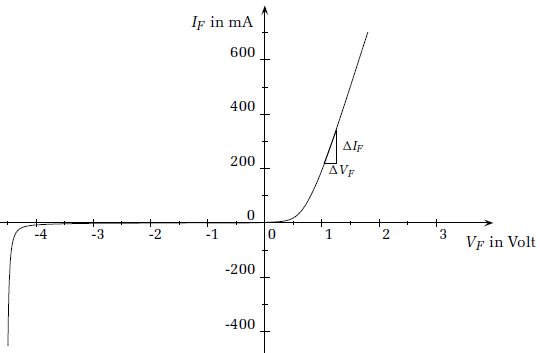
\includegraphics[width=6cm]{bilder/DiodenKennlinie}
	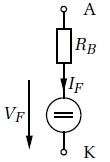
\includegraphics[width=3cm]{bilder/DiodenKleinsignal}\\
	$g = \frac{1}{R}= \frac{\Delta I}{\Delta V}$
	\columnbreak
	
	\section{Transitoren}
		\subsection{Transistortypen}
		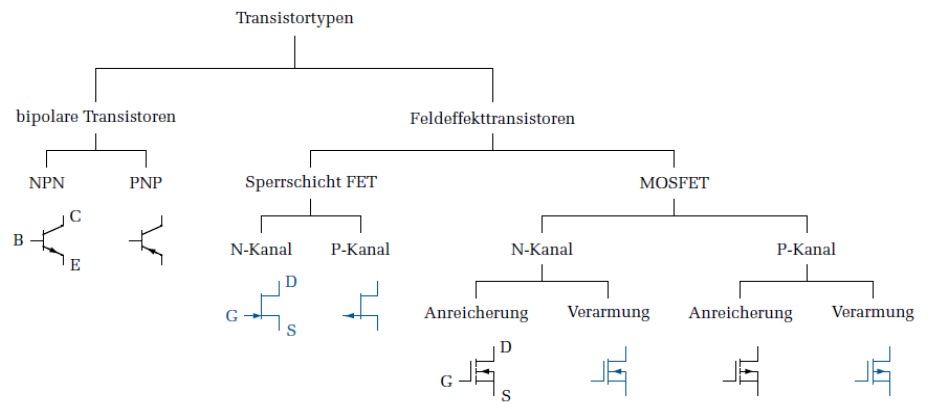
\includegraphics[width=9cm]{bilder/Transistortypen.png}
\end{multicols}

\subsection{Bipolartransistoren}
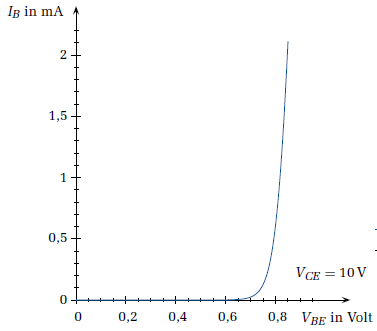
\includegraphics[width=5.5cm]{bilder/bipolarEingangsKennlinie}
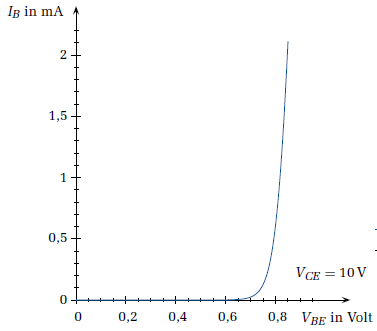
\includegraphics[width=5.5cm]{bilder/bipolarVerstaerkungsKennlinie}
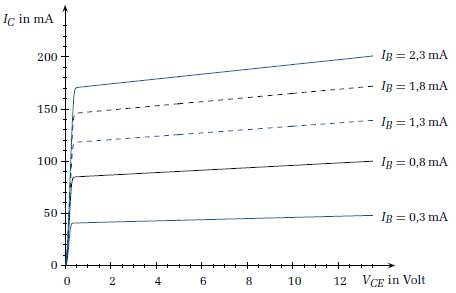
\includegraphics[width=7cm]{bilder/bipolarAusgangsKennlinie}\\
\begin{tabular}{ll}
	Wechselstromverstärkung $\beta = \frac{\Delta I_B}{\Delta I_B} $&
	Gleichstromverstärkung $B = \frac{I_C}{I_B}$\\
\end{tabular}

\subsection{Feldeffekt-Transistoren}

\subsubsection{n-Kanal-JFET}
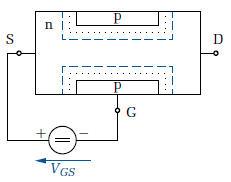
\includegraphics[width=5cm]{bilder/jFET}
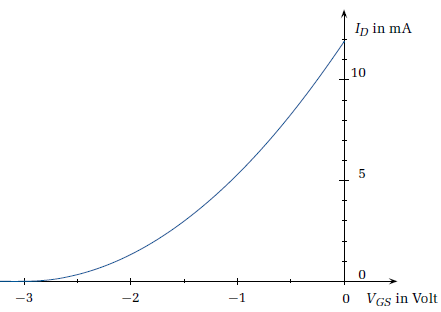
\includegraphics[width=6cm]{bilder/jFetSteuerKennlinie}
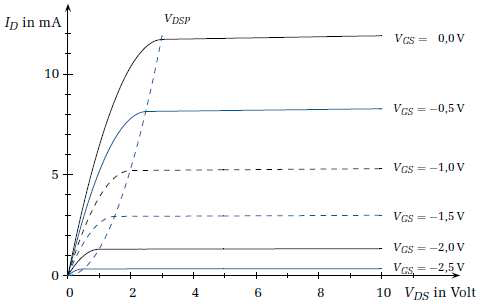
\includegraphics[width=6cm]{bilder/jFetAusgangsKennlinie}\\

\subsubsection{n-Kanal MOSFET}

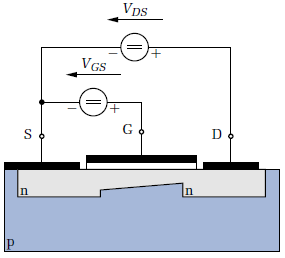
\includegraphics[width=5cm]{bilder/MOSFET}
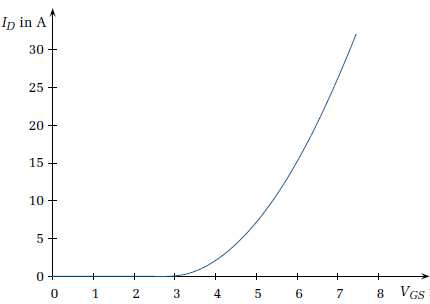
\includegraphics[width=6cm]{bilder/MOSFETSteuerKennlinie}
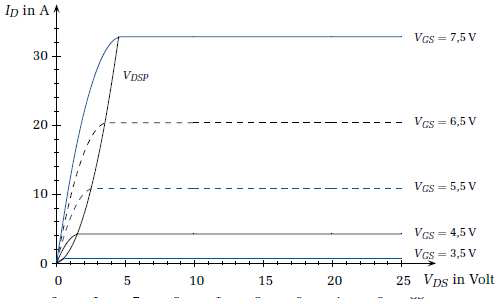
\includegraphics[width=6cm]{bilder/MOSFETAusgangsKennlinie}\\
